\section{Дополнительные эксперименты} \label{Appendix}

    В этом разделе приводятся результаты эксперимента~\ref{exp_2}, который заключался в анализе невязок на нормальность, и эксперимента~\ref{exp_3}, в котором проверялись предсказания Теоремы~\ref{delta} для модели Ridge на синтетическом наборе данных и наборе данных Фридмана.

    \begin{figure}[ht]
        \centering
        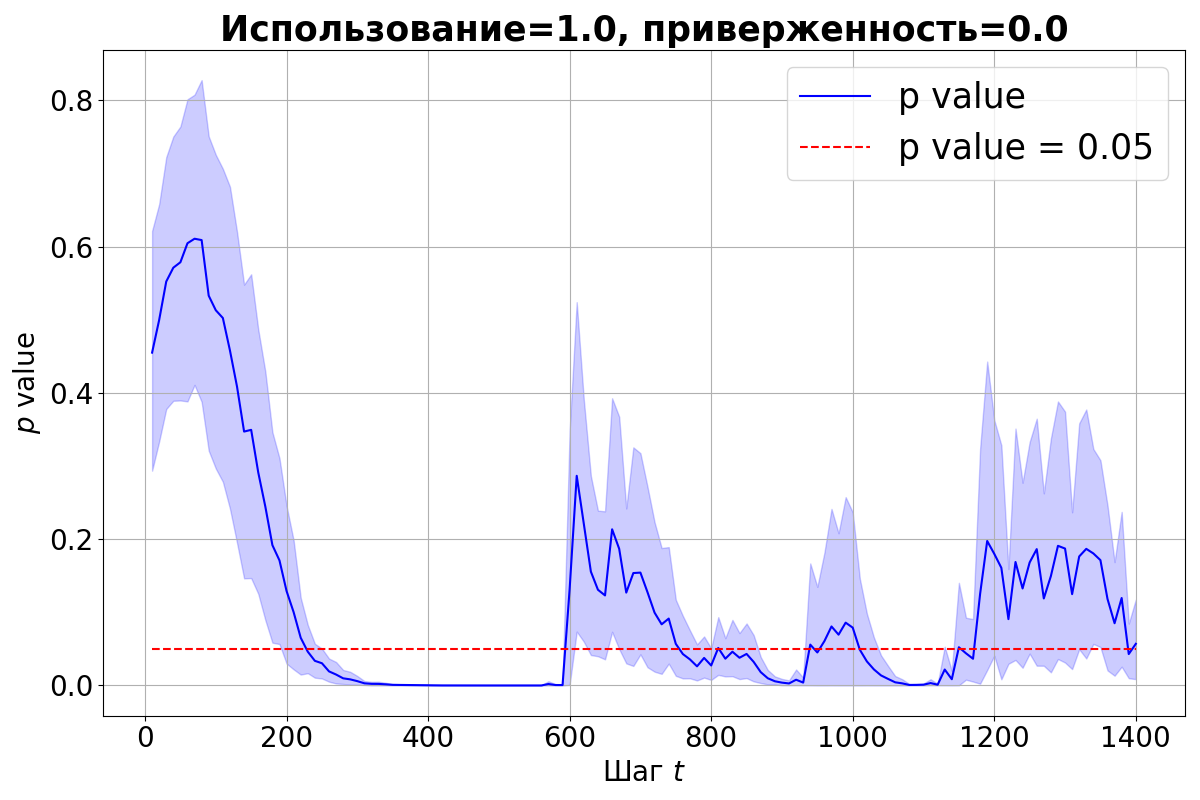
\includegraphics[width=0.49\linewidth]{pictures/p_sw_synthetic_sgd_model_50_1.0_0.0.png}
        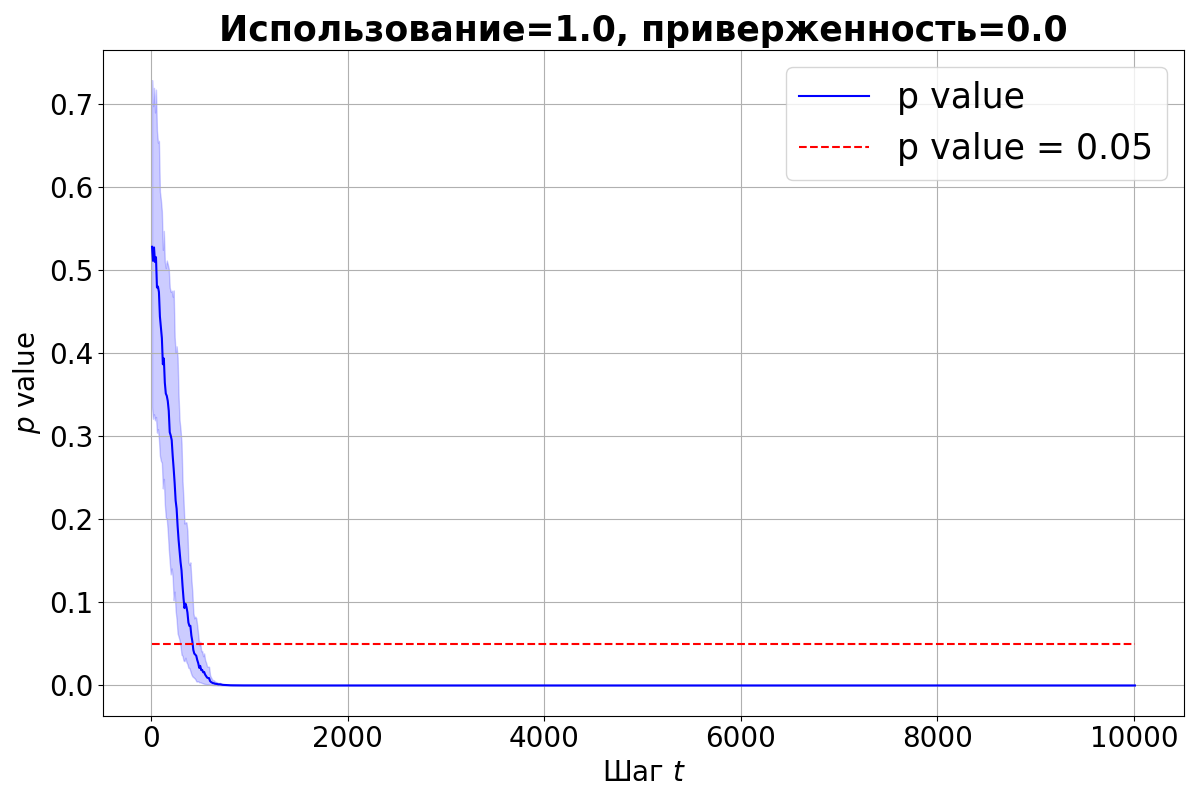
\includegraphics[width=0.49\linewidth]{pictures/p_su_synthetic_sgd_model_50_1.0_0.0.png}
        
        \caption{Проверка распределения невязок модели на нормальность со временем для регрессионной модели SGD на линейном наборе данных. Скользящее окно (слева), обновление выборки (справа).}
        \label{p_value}
    \end{figure}

    Как видно из Рис.~\ref{p_value}, $p$-value со временем становится меньше $0,05$, то есть нормальность невязок нарушается.

    \begin{figure}[ht]
        \centering
        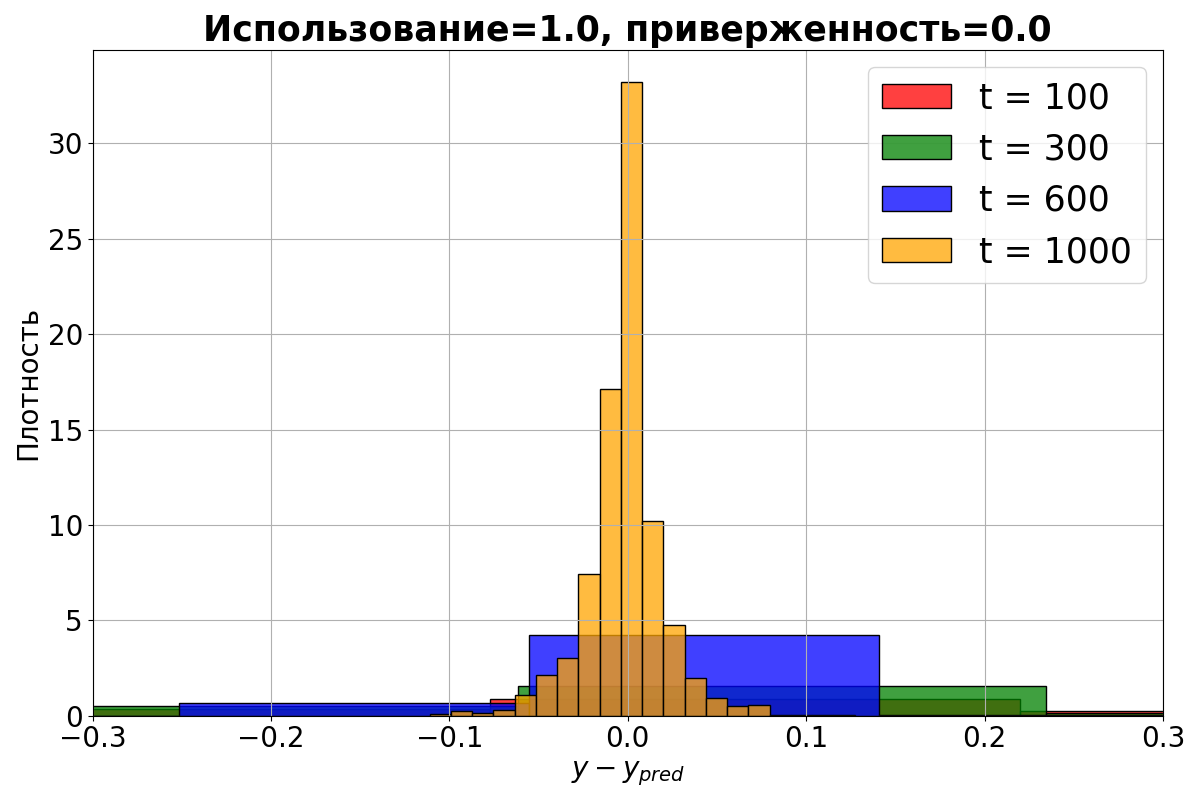
\includegraphics[width=0.49\linewidth]{pictures/hist_sw_synthetic_sgd_model_50_1.0_0.0.png}
        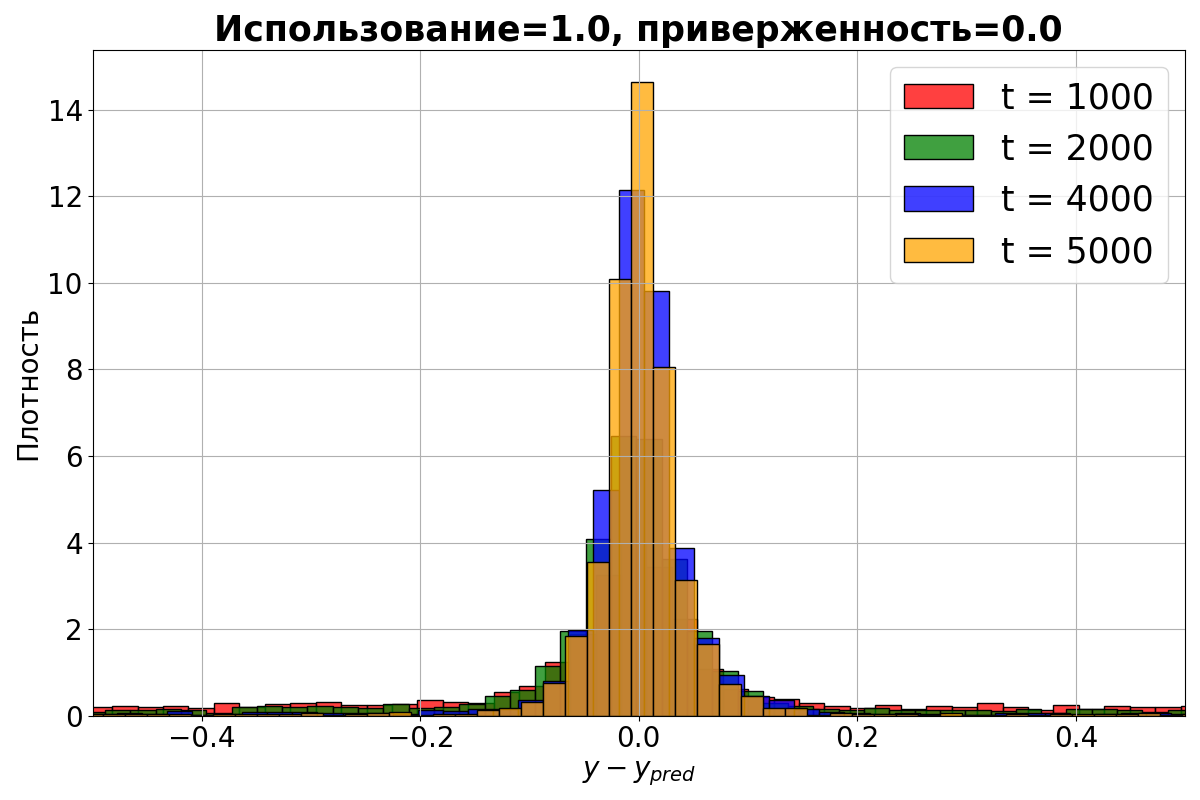
\includegraphics[width=0.49\linewidth]{pictures/hist_su_synthetic_sgd_model_50_1.0_0.0.png}
        
        \caption{Гистограммы невязок модели со временем для регрессионной модели SGD на линейном наборе данных.Скользящего окно (слева), Обновление выборки (справа).}
        \label{hist}
    \end{figure}

    Из Рис.~\ref{hist} можно сделать вывод, что $\mathbf{y} - \mathbf{y'}$ -- это смесь двух распределений.

    \begin{figure}
        \centering
        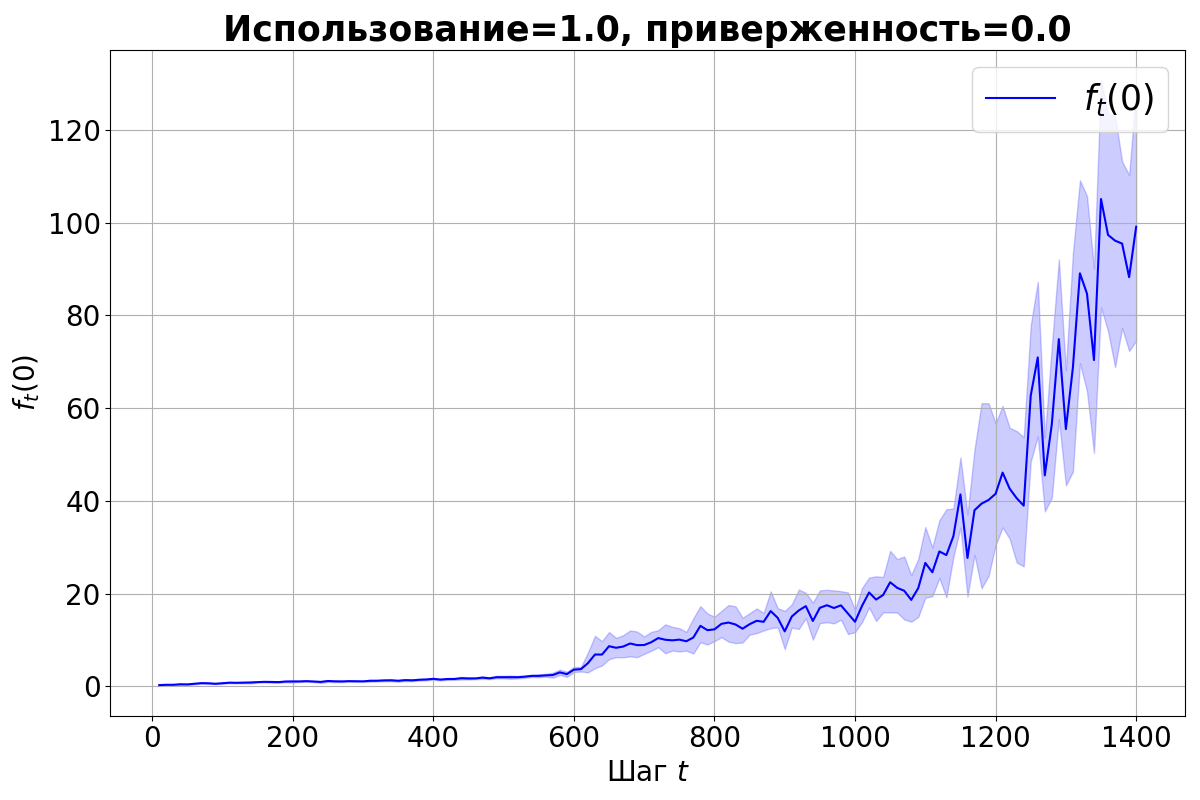
\includegraphics[width=0.32\linewidth]{pictures/ft0_sw_friedman_ridge_model_0.0_1.0_0.0.png}~
        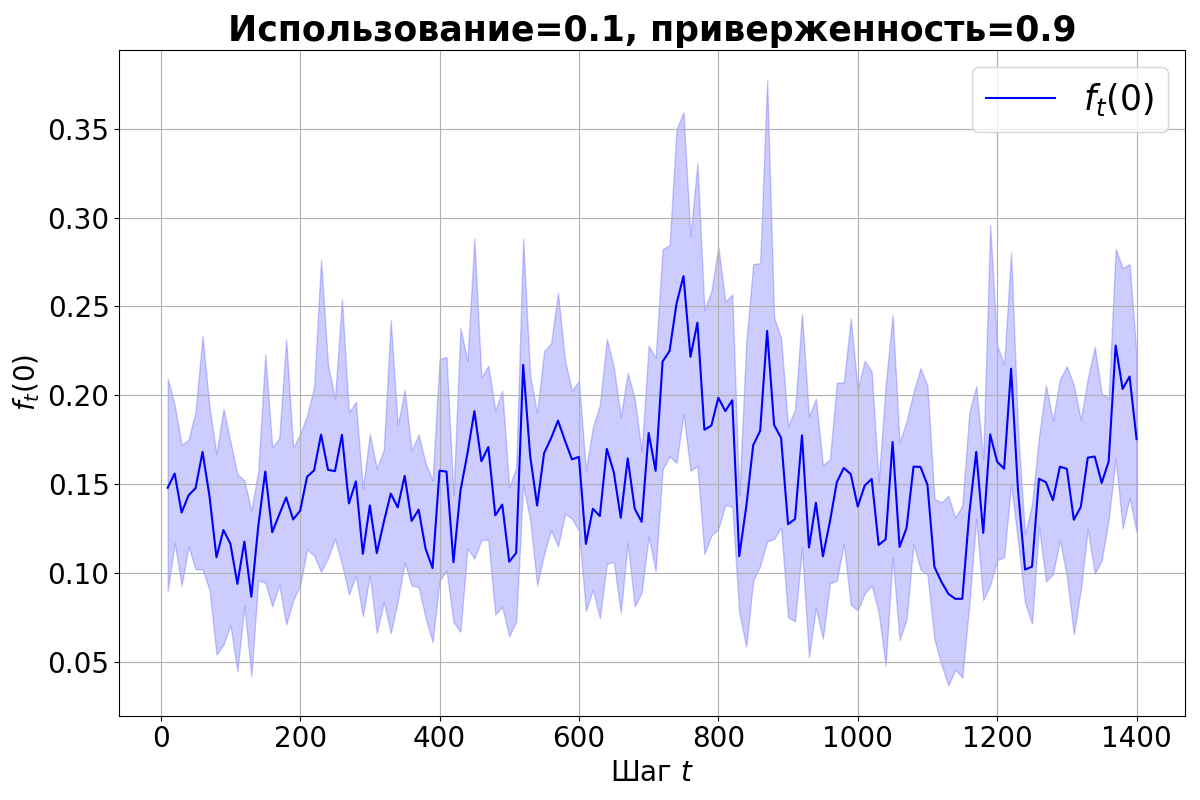
\includegraphics[width=0.32\linewidth]{pictures/ft0_sw_friedman_ridge_model_0.0_0.1_0.9.png}~
        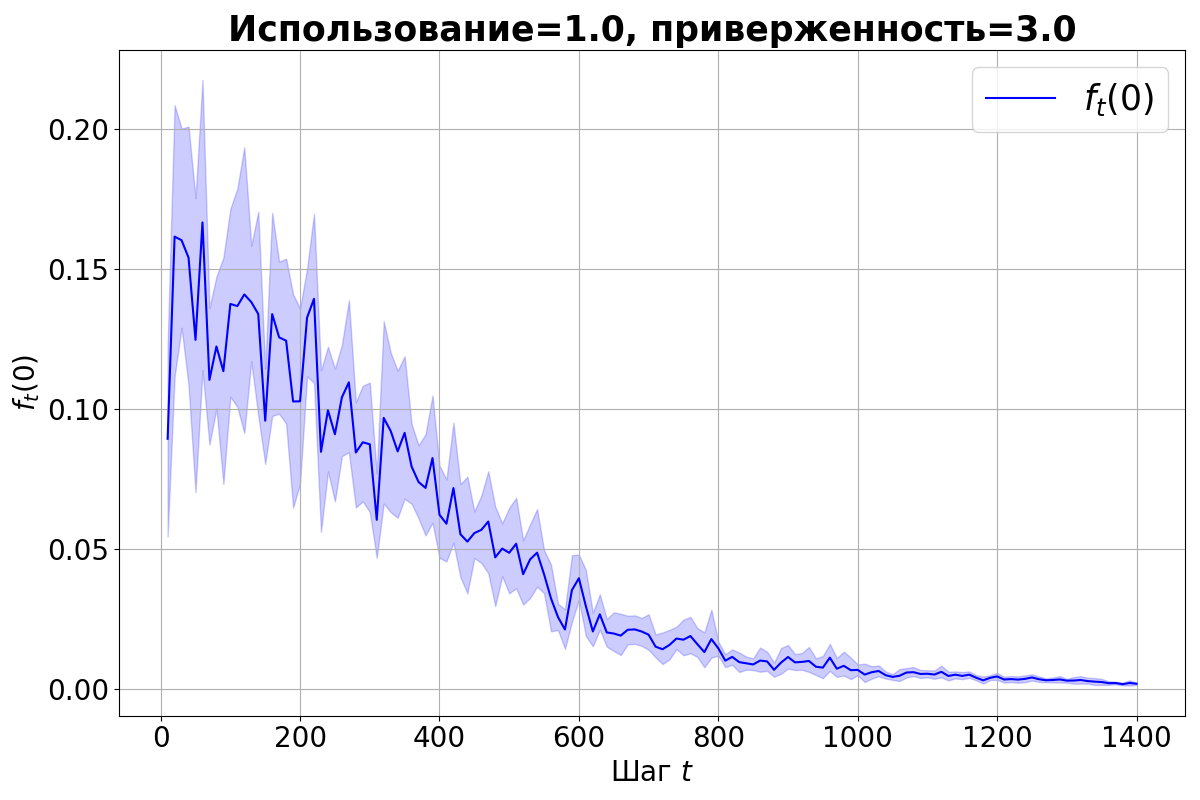
\includegraphics[width=0.32\linewidth]{pictures/ft0_sw_friedman_ridge_model_0.0_1.0_3.0.png}
    
        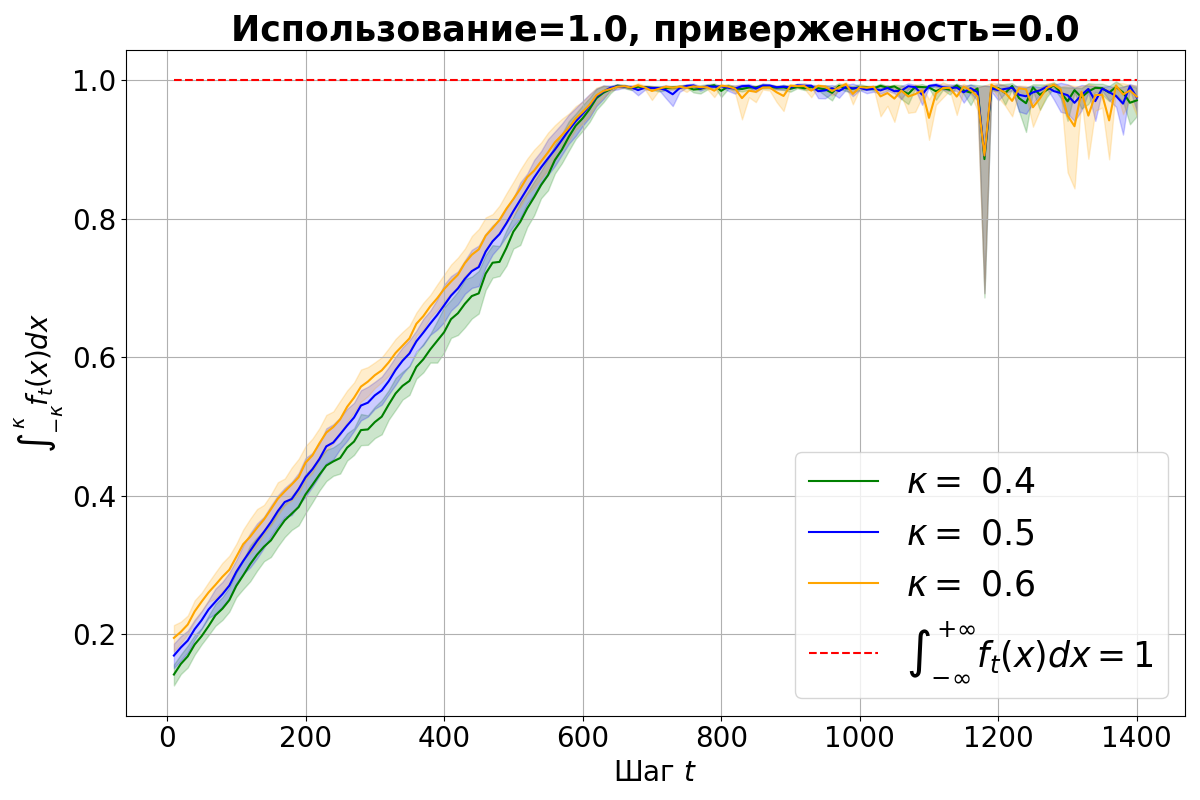
\includegraphics[width=0.32\linewidth]{pictures/int_sw_friedman_ridge_model_0.0_1.0_0.0.png}~
        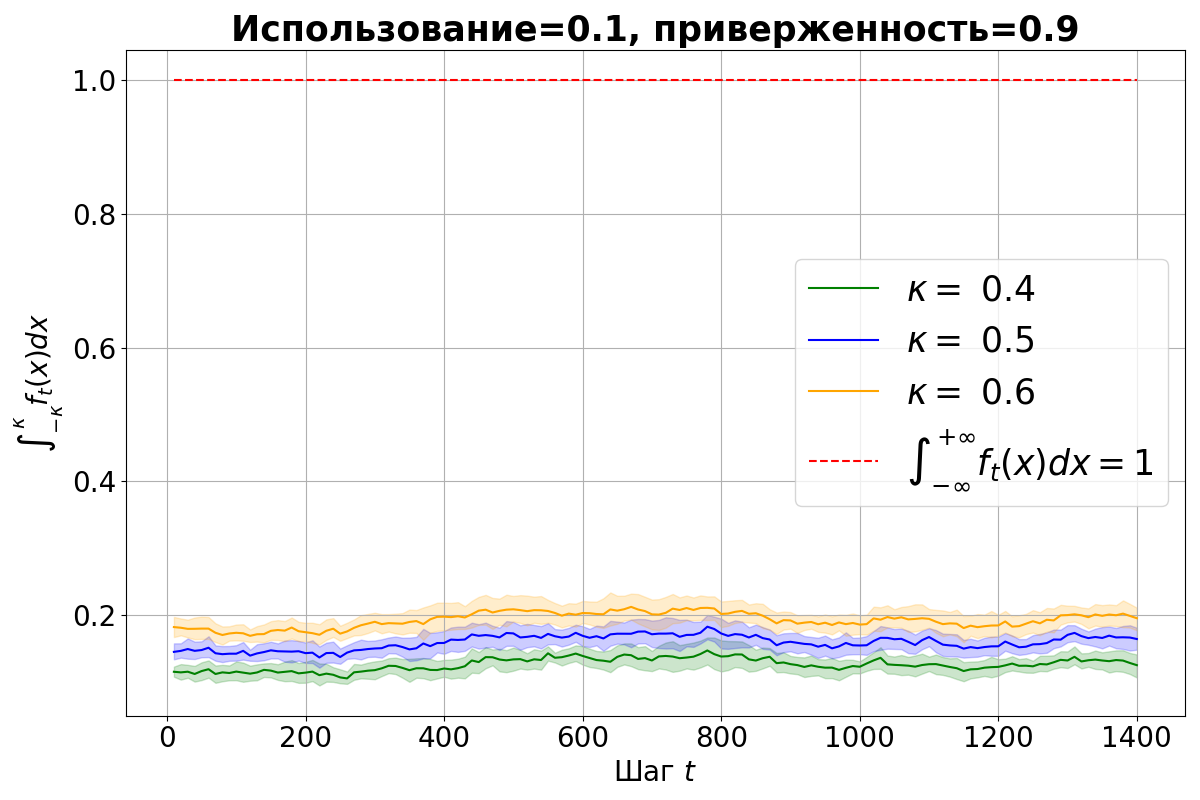
\includegraphics[width=0.32\linewidth]{pictures/int_sw_friedman_ridge_model_0.0_0.1_0.9.png}~
        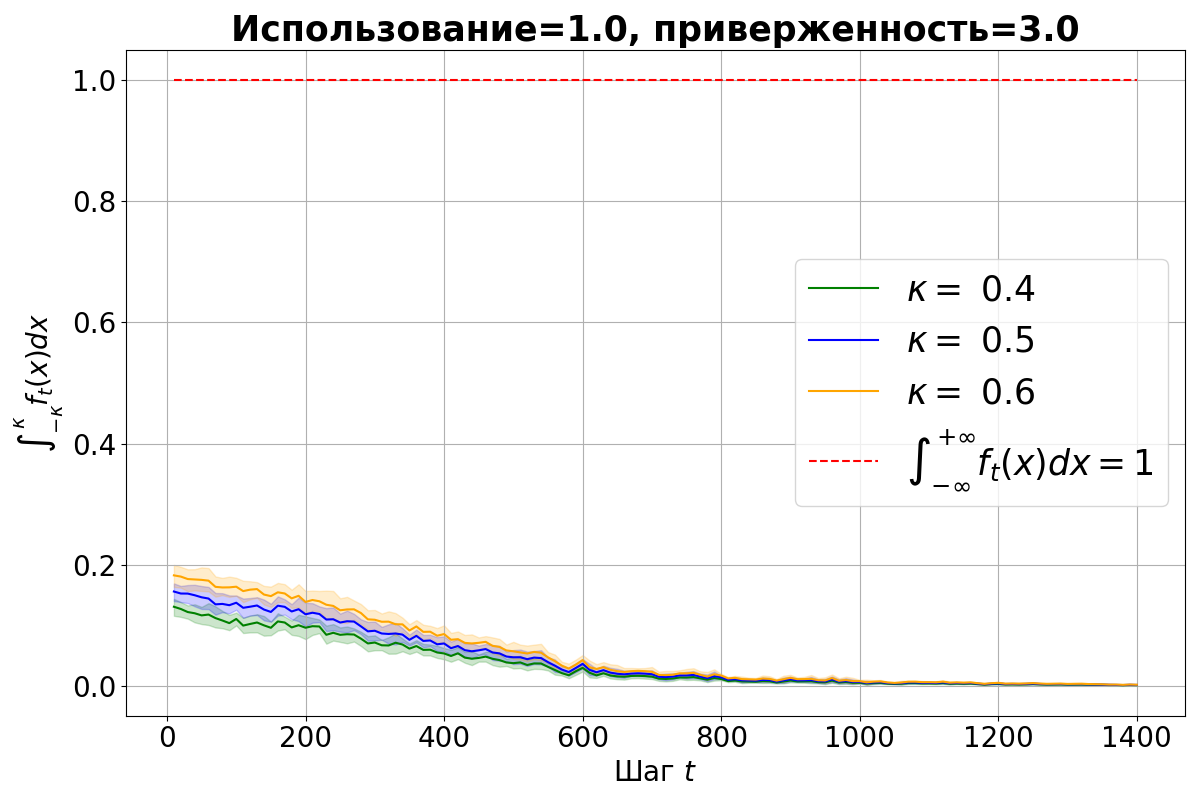
\includegraphics[width=0.32\linewidth]{pictures/int_sw_friedman_ridge_model_0.0_1.0_3.0.png}
        
        \caption{Вычисление $f_t(0)$ и $\int_{-\kappa}^{\kappa}f_t(x)dx$ в постановке скользящее окно для модели Ridge на наборе данных Фридмана. Рассматриваются: использование, приверженность = $1$, $0$ (слева); $0,1$, $0,9$ (посередине); $1$, $3$ (справа). На этом рисунке виды все предельное множество системы \eqref{system} из Теоремы~\ref{delta}.}
        \label{delta_loop_1}
    \end{figure}

    \begin{figure}
        \centering
        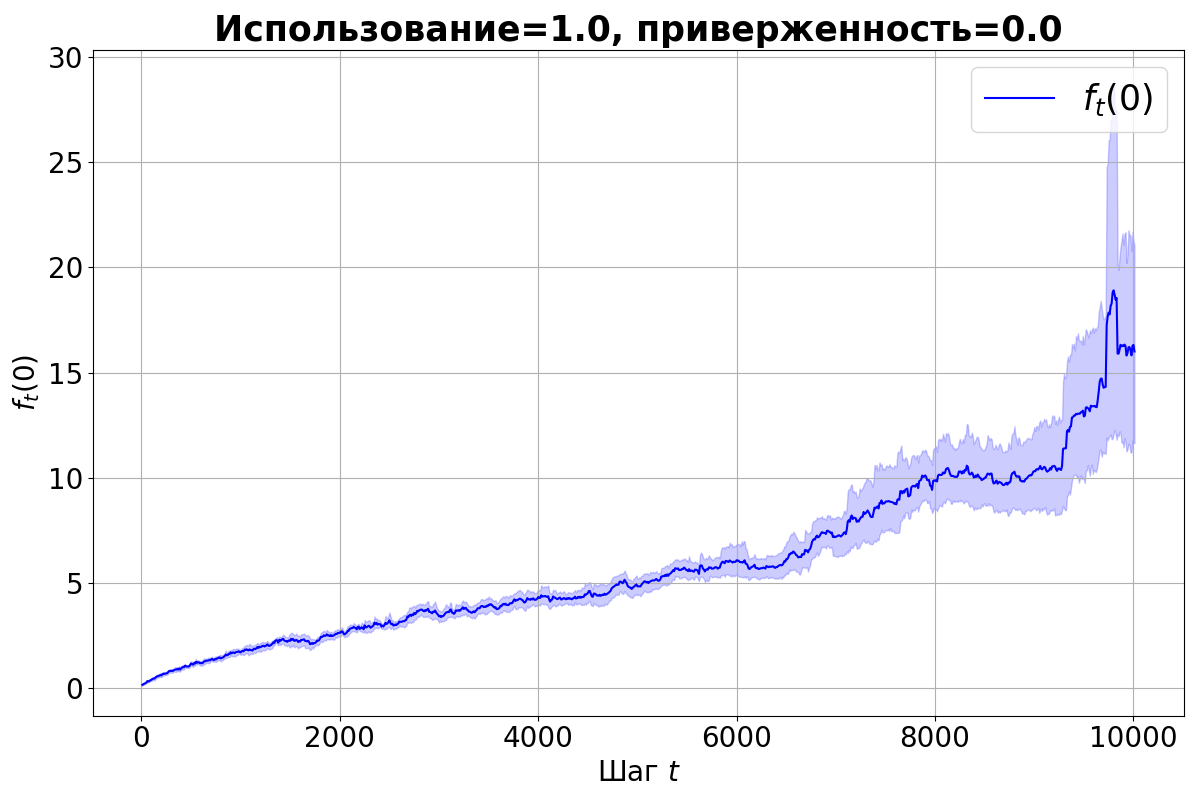
\includegraphics[width=0.32\linewidth]{pictures/ft0_su_friedman_ridge_model_0.0_1.0_0.0.png}~
        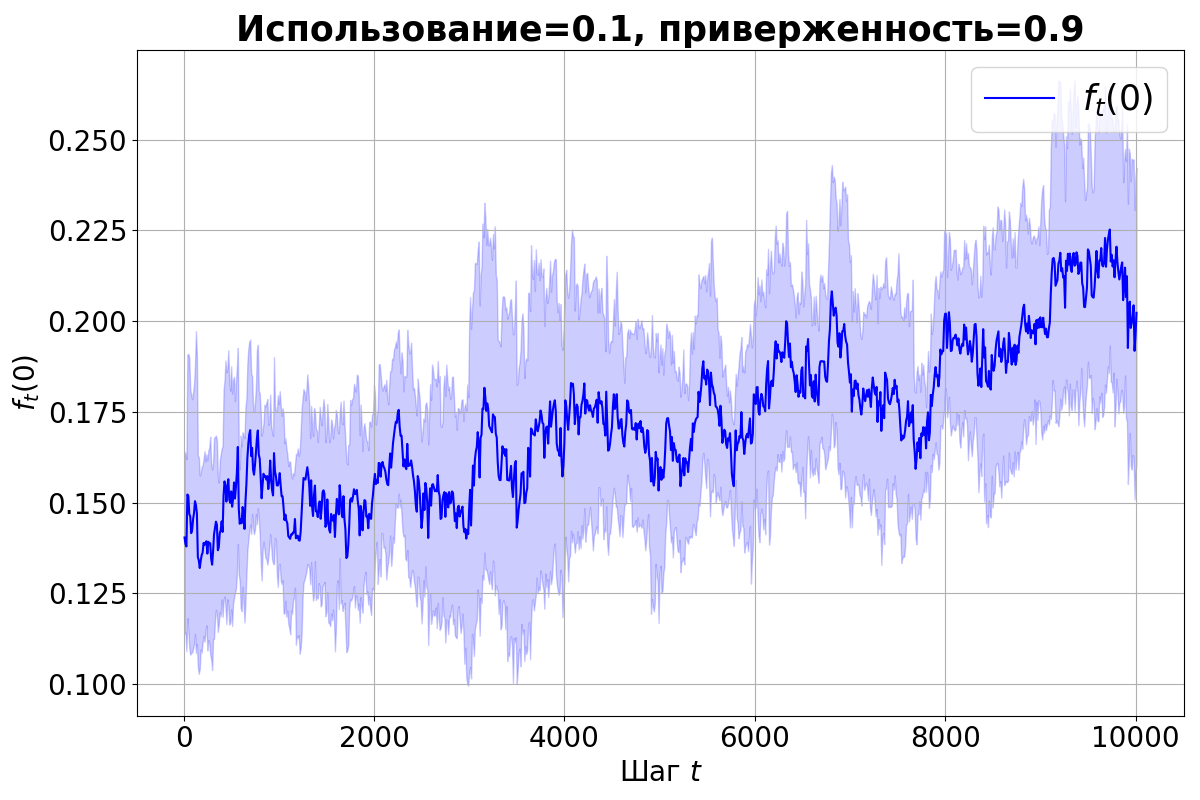
\includegraphics[width=0.32\linewidth]{pictures/ft0_su_friedman_ridge_model_0.0_0.1_0.9.png}~
        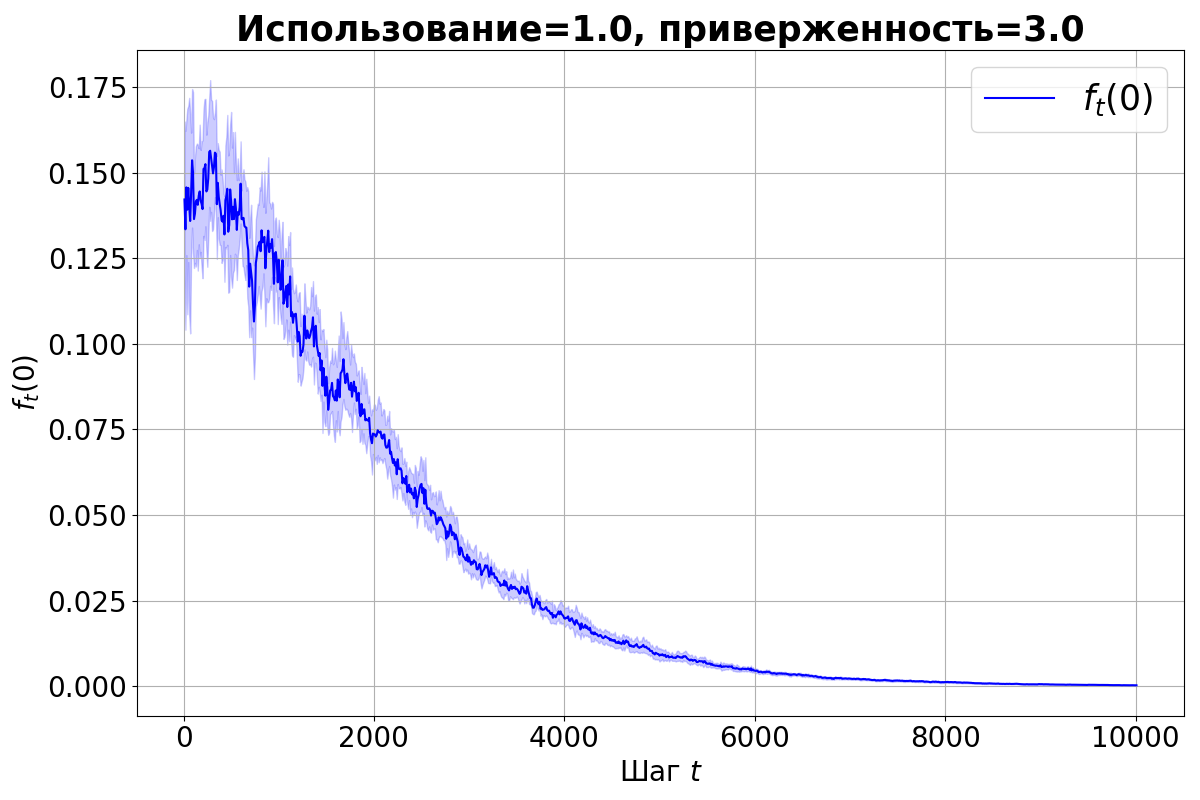
\includegraphics[width=0.32\linewidth]{pictures/ft0_su_friedman_ridge_model_0.0_1.0_3.0.png}

        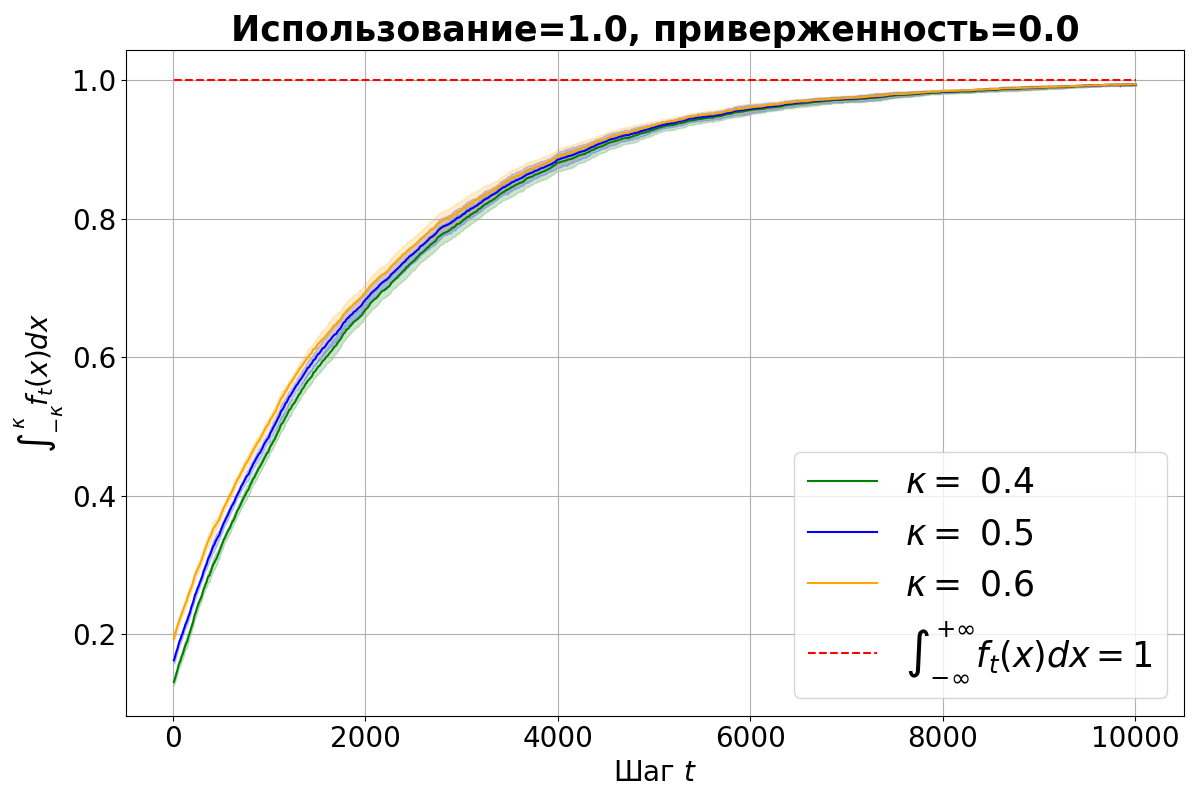
\includegraphics[width=0.32\linewidth]{pictures/int_su_friedman_ridge_model_0.0_1.0_0.0.png}~
        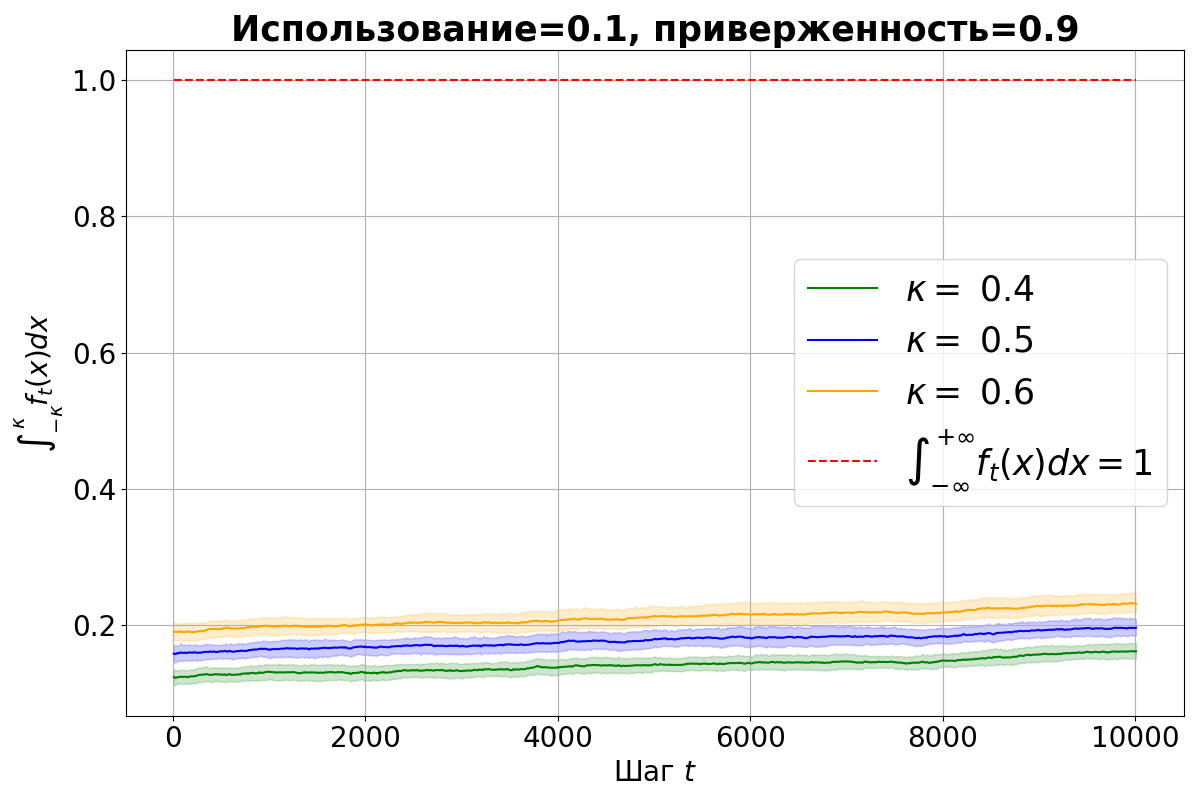
\includegraphics[width=0.32\linewidth]{pictures/int_su_friedman_ridge_model_0.0_0.1_0.9.png}~
        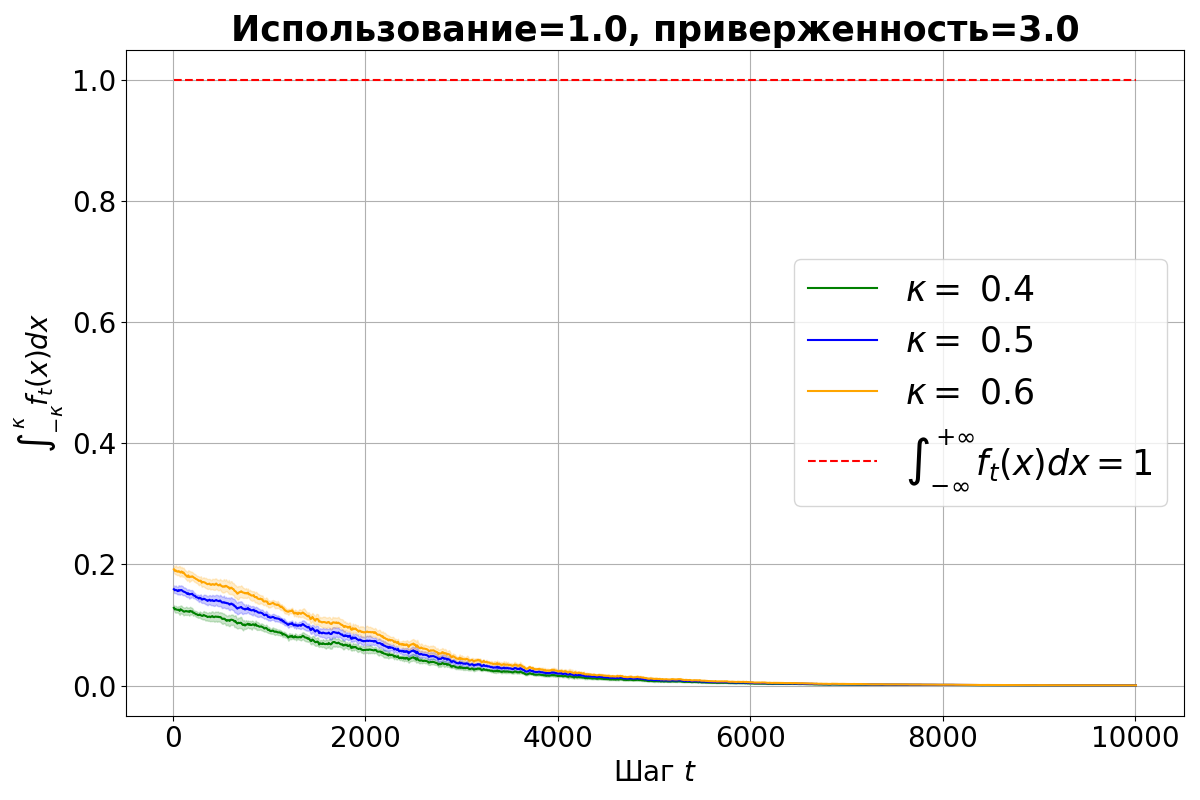
\includegraphics[width=0.32\linewidth]{pictures/int_su_friedman_ridge_model_0.0_1.0_3.0.png}
        
        \caption{Вычисление $f_t(0)$ и $\int_{-\kappa}^{\kappa}f_t(x)dx$ в постановке обновление выборки для модели Ridge на наборе данных Фридмана. Рассматриваются: использование, приверженность = $1$, $0$ (слева); $0,1$, $0,9$ (посередине); $1$, $3$ (справа). На этом рисунке виды все предельное множество системы \eqref{system} из Теоремы~\ref{delta}.}
        \label{delta_sample_1}
    \end{figure}

    Результаты, приведенные на Рис.~\ref{delta_loop_1}~и~\ref{delta_sample_1} аналогичны Рис.~\ref{delta_loop}~и~\ref{delta_sample}, поэтому можно сделать вывод, что результаты Теоремы~\ref{delta} обобщаются на различные наборы данных и модели машинного обучения.